\documentclass[12pt]{exam}
\usepackage{xparse}
\usepackage{rosoff-vector-macros}
\usepackage{rosoff}
\usepackage{graphicx}
\DeclareGraphicsExtensions{.jpg, .png}
\usepackage{fourier}
\usepackage{MnSymbol}
\usepackage{amsthm}
\usepackage{paralist,enumerate,listings}
\usepackage{siunitx}
\frenchspacing
\usepackage{parskip}
\usepackage{hyperref}
\firstpageheader{}{}{}
\runningheader{\textbf{Fall 2013}}
 {}
 {\textbf{Math 251}}
 %{\emph{Page \thepage~of \numpages}}
\runningheadrule

\pagestyle{head}

\begin{document}
\noindent
\textbf{{\large Math 251 \hfill Quiz 10}}
% \hfill Name: \underline{\hspace{0.5in}Answers\hspace{2in}}

\noindent
December 6, 2013; 10 minutes \hfill Name: \underline{\hspace{3in}} 

\noindent

\noindent
This quiz is \emph{open-note}, but no books or calculators may be used.
You don't need to give any justification for your answers.

\begin{questions} 

    \question[6] Suppose $\vec{F}(x,y) = \angl{6y \sin{(xy)}, 6x \sin{(xy)}}$ and $\mathcal{C}$ is the segment of the parabola $y = 2x^2$ from the point $(1,2)$ to $(4,32)$. Find the value of  $\int_{\mathcal{C}} \vec{F} \cdot d\vec{s}$. (Note that this is the same as $\int_{\mathcal{C}} \vec{F} \cdot d\vec{r}$.)

    \dwrspace{1}

    \question Consider the vector field $\vec{F}$ and closed path $\mathcal{C}$ as in the figure.
    \begin{figure}[ht]
        \begin{minipage}[t]{0.4\textwidth}
            \vspace{0pt}
            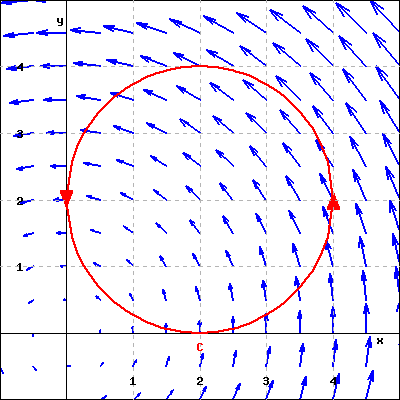
\includegraphics[width=\linewidth,height=\linewidth]{images/image.png}
        \end{minipage} \hspace{1em}
        \begin{minipage}[t]{0.4\textwidth}
            \vspace{0pt}
            \begin{parts}
                \part[3] Is $\int_{\mathcal{C}} \vec{F} \cdot d\vec{s}$ positive, negative, or zero?

                \vspace{1.5in}

                \part[3] True or false: $\vec{F}$ is a conservative vector field.
            \end{parts}
        \end{minipage}
    \end{figure}

    \dwrspace{1}

\end{questions} 

\end{document}